%% ViACaPu — IEEE Conference Paper (IEEEtran, English)
%% Compile: pdflatex paper_ieee.tex  (twice for references)
%% Figures: place the figures/ folder next to this .tex file.
\documentclass[conference]{IEEEtran}
\IEEEoverridecommandlockouts

\usepackage{cite}
\usepackage{amsmath,amssymb,amsfonts}
\usepackage{graphicx}
\usepackage{textcomp}
\usepackage{xcolor}
\usepackage{booktabs}
\usepackage{multirow}
\usepackage[utf8]{inputenc}
\usepackage[T1]{fontenc}

\begin{document}

\title{ViACaPu: A Lightweight Acoustic-Aware Model for\\
Punctuation and Casing Restoration in On-Device Streaming ASR}

\author{\IEEEauthorblockN{Nguyen Doan Sy, Ngoc Mai Xuan, Vinh La The,
Hiep Hoang Van, Hung Pham Ngoc, Thuan Nguyen Dinh}
\IEEEauthorblockA{\textit{Hanoi University of Science and Technology}\\
Ha Noi, Vietnam}
}

\maketitle

\begin{abstract}
Punctuation and word-casing restoration (CaPu) is an essential post-processing
step that renders automatic speech recognition (ASR) output readable. Current
high-quality CaPu models rely on large pretrained Transformers with hundreds of
millions of parameters, unsuitable for edge deployment, whereas lightweight
text-only models are bounded by a quality ceiling because they lack prosodic
evidence---pauses and intonation that mark clause and sentence boundaries. We
propose \textbf{ViACaPu}, a lightweight multimodal CaPu model (3.58M parameters)
that couples a compact text branch with a small log-Mel acoustic branch through
\emph{gated cross-attention}. The fusion is \emph{alignment-free}: word
representations softly attend to acoustic frames without word-level timestamps, so
the module can be attached to any existing ASR system. On the Vietnamese
Dolly-1000h corpus, ViACaPu attains \textbf{0.921} punctuation F1 and
\textbf{0.943} casing F1, improving an identically-configured text-only ablation by
\textbf{+0.099} absolute punctuation F1 and \textbf{+0.212} comma F1 at only 0.91M
additional parameters. Notably, the proposed model is also \emph{smaller} than the
text-only baseline it is compared against (3.58M vs.\ 7.26M) while scoring
substantially higher, making high-quality CaPu practical for on-device streaming
ASR.
\end{abstract}

\begin{IEEEkeywords}
punctuation restoration, word casing, on-device ASR, acoustic-textual fusion,
cross-attention, low-resource speech processing
\end{IEEEkeywords}

\section{Introduction}

Modern ASR systems emit unpunctuated, lowercase word sequences. Restoring
punctuation and casing (CaPu) is therefore required before the transcript is read
by humans or consumed by downstream components such as machine translation or
summarisation~\cite{survey}.

Two solution families dominate. \emph{Text-only} models treat CaPu as sequence
labelling over the recognised words; the strongest variants fine-tune large
pretrained language models (e.g.\ BERT~\cite{bertpunct}), whose size (often
$>$100M parameters) precludes on-device execution. \emph{End-to-end} approaches fold punctuation prediction into
the acoustic model, but require retraining the whole ASR and cannot be attached to
an already deployed recogniser.

Recently, You and Li~\cite{you2024lightweight} showed that a compact CNN--BiLSTM
architecture achieves competitive punctuation quality at a fraction of the size of
Transformer baselines, making CaPu feasible on-device. That model, however, remains
\emph{text-only}, forfeiting the prosodic evidence naturally present in speech:
commas frequently co-occur with pauses, and questions with a rising terminal
contour. Our error analysis confirms that the comma class is by far the weakest for
text-only models.

Our goal is a \emph{lightweight yet high-quality} Vietnamese CaPu model suitable
for on-device streaming ASR. We realise it with \textbf{ViACaPu}, whose
contributions are:

\begin{itemize}
\item A lightweight CaPu model (only 3.58M parameters, Section~\ref{sec:method})
      that reaches high quality on Vietnamese while being smaller than---and
      scoring markedly above---the text-only baseline it is compared against.
\item A key method for the quality gain: \emph{acoustic evidence fusion} via
      alignment-free gated cross-attention. On Vietnamese it lifts punctuation F1
      $0.822 \rightarrow 0.921$ and comma F1 $0.661 \rightarrow 0.873$ at
      $+0.91$M parameters, relative to the same model with the acoustic branch
      disabled.
\item A detailed error analysis (Section~\ref{sec:results}) showing that the gain
      is concentrated precisely where prosody is informative: comma recall rises
      from 0.659 to 0.892, while casing---a predominantly lexical
      phenomenon---remains essentially unchanged.
\end{itemize}

\section{Related Work}

\textbf{Text-only CaPu.} The standard approach is sequence labelling over the
recognised words. The lightweight CNN--BiLSTM model of You and
Li~\cite{you2024lightweight}, which our text branch follows, predicts casing from
left context and punctuation from right context by concatenating adjacent word
states, deliberately avoiding self-attention, which the authors report to yield
degenerate outputs. Transformer- and PLM-based systems reach higher accuracy at
substantially larger model size.

\textbf{Acoustic and multimodal CaPu.} Prosodic features (pause duration, $F_0$,
energy) have long been known to correlate with punctuation, and recent work
confirms that combining text with acoustic evidence improves punctuation
prediction over text-only models~\cite{cho2022,tran2020}. Notably, Cho \emph{et
al.}~\cite{cho2022} fuse pause, $F_0$ and energy features with text and conclude
that \emph{commas are the hardest class to predict}---matching our own error
analysis (Section~\ref{sec:results}). Closest to ours, UniPunc~\cite{unipunc}
fuses
lexical and acoustic features via self-attention and \emph{cross-attention} in a
shared latent space, showing cross-attention to be an effective fusion mechanism;
however UniPunc relies on a BERT encoder (768-dim), whose size is unsuited to the
edge. In a different direction, end-to-end \emph{speech-to-punctuated-text} (STPT)
systems train the ASR to emit punctuated text directly~\cite{stpt}, but this
requires retraining the whole recogniser and cannot be attached to a deployed one.
Notably, Jakubiak \emph{et al.}~\cite{stpt} observe that models using acoustic
features are \emph{usually bigger and more complex} than purely lexical ones---the
exact gap ViACaPu fills: it exploits prosody yet stays lightweight. Unlike both
directions, ViACaPu is a standalone, lightweight post-processing module that
consumes only the recognised text and the log-Mel features any ASR front end
already computes.

\textbf{Lightweight CaPu for streaming ASR.} Several recent works target online,
lightweight CaPu for streaming ASR, e.g.\ using a small ELECTRA
model~\cite{polacek2023} or compact online models~\cite{lightweight2025};
end-to-end systems also fold punctuation into streaming ASR~\cite{kim2023}, and
LibriSpeech-PC~\cite{librispeechpc} provides a benchmark for the punctuation and
casing capabilities of end-to-end ASR. These, however, are either text-only or
tightly coupled to the ASR; ViACaPu adds acoustic evidence as a standalone module.

\textbf{Casing restoration.} Casing is usually handled jointly with punctuation:
Nguyen \emph{et al.}~\cite{nguyen2019} use a Transformer with overlapped chunk
merging to restore both in a single pass, and Sunkara \emph{et
al.}~\cite{sunkara2020} robustly predict punctuation and truecasing for medical
ASR. Our casing branch inherits the adjacent-state concatenation
of~\cite{you2024lightweight}.

\textbf{CaPu for Vietnamese.} For Vietnamese, JointCapPunc~\cite{jointcappunc}
proposes a joint multi-task model built on a pretrained Transformer encoder
(XLM-R/vELECTRA) and releases a public dataset. It attains high quality but uses a
hundreds-of-millions-parameter encoder; the authors themselves note that this scale
raises latency concerns in an ASR pipeline and list model shrinking as future work.
To our knowledge, ViACaPu is the first \emph{acoustic-aware, lightweight} CaPu model
for Vietnamese.

\textbf{Limitations of prior work and our motivation.} The analysis above reveals
three gaps. (i)~PLM/Transformer models achieve high quality but are \emph{too heavy}
for the edge. (ii)~The lightweight text-only model~\cite{you2024lightweight} is
device-feasible but \emph{ignores acoustic evidence}, imposing a quality ceiling on
the comma class---which, as Section~\ref{sec:results} shows, depends strongly on
speech pauses. (iii)~End-to-end systems exploit prosody but \emph{require retraining
the entire ASR}. ViACaPu resolves all three at once: it keeps the light footprint
of (ii), adds acoustic evidence like (iii), but as a \emph{standalone,
alignment-free post-processing module}---cross-attention learns a soft alignment
between word states and acoustic frames, making it portable across recognisers
without word-level timestamps.

\section{Method}
\label{sec:method}

\begin{figure}[t]
\centerline{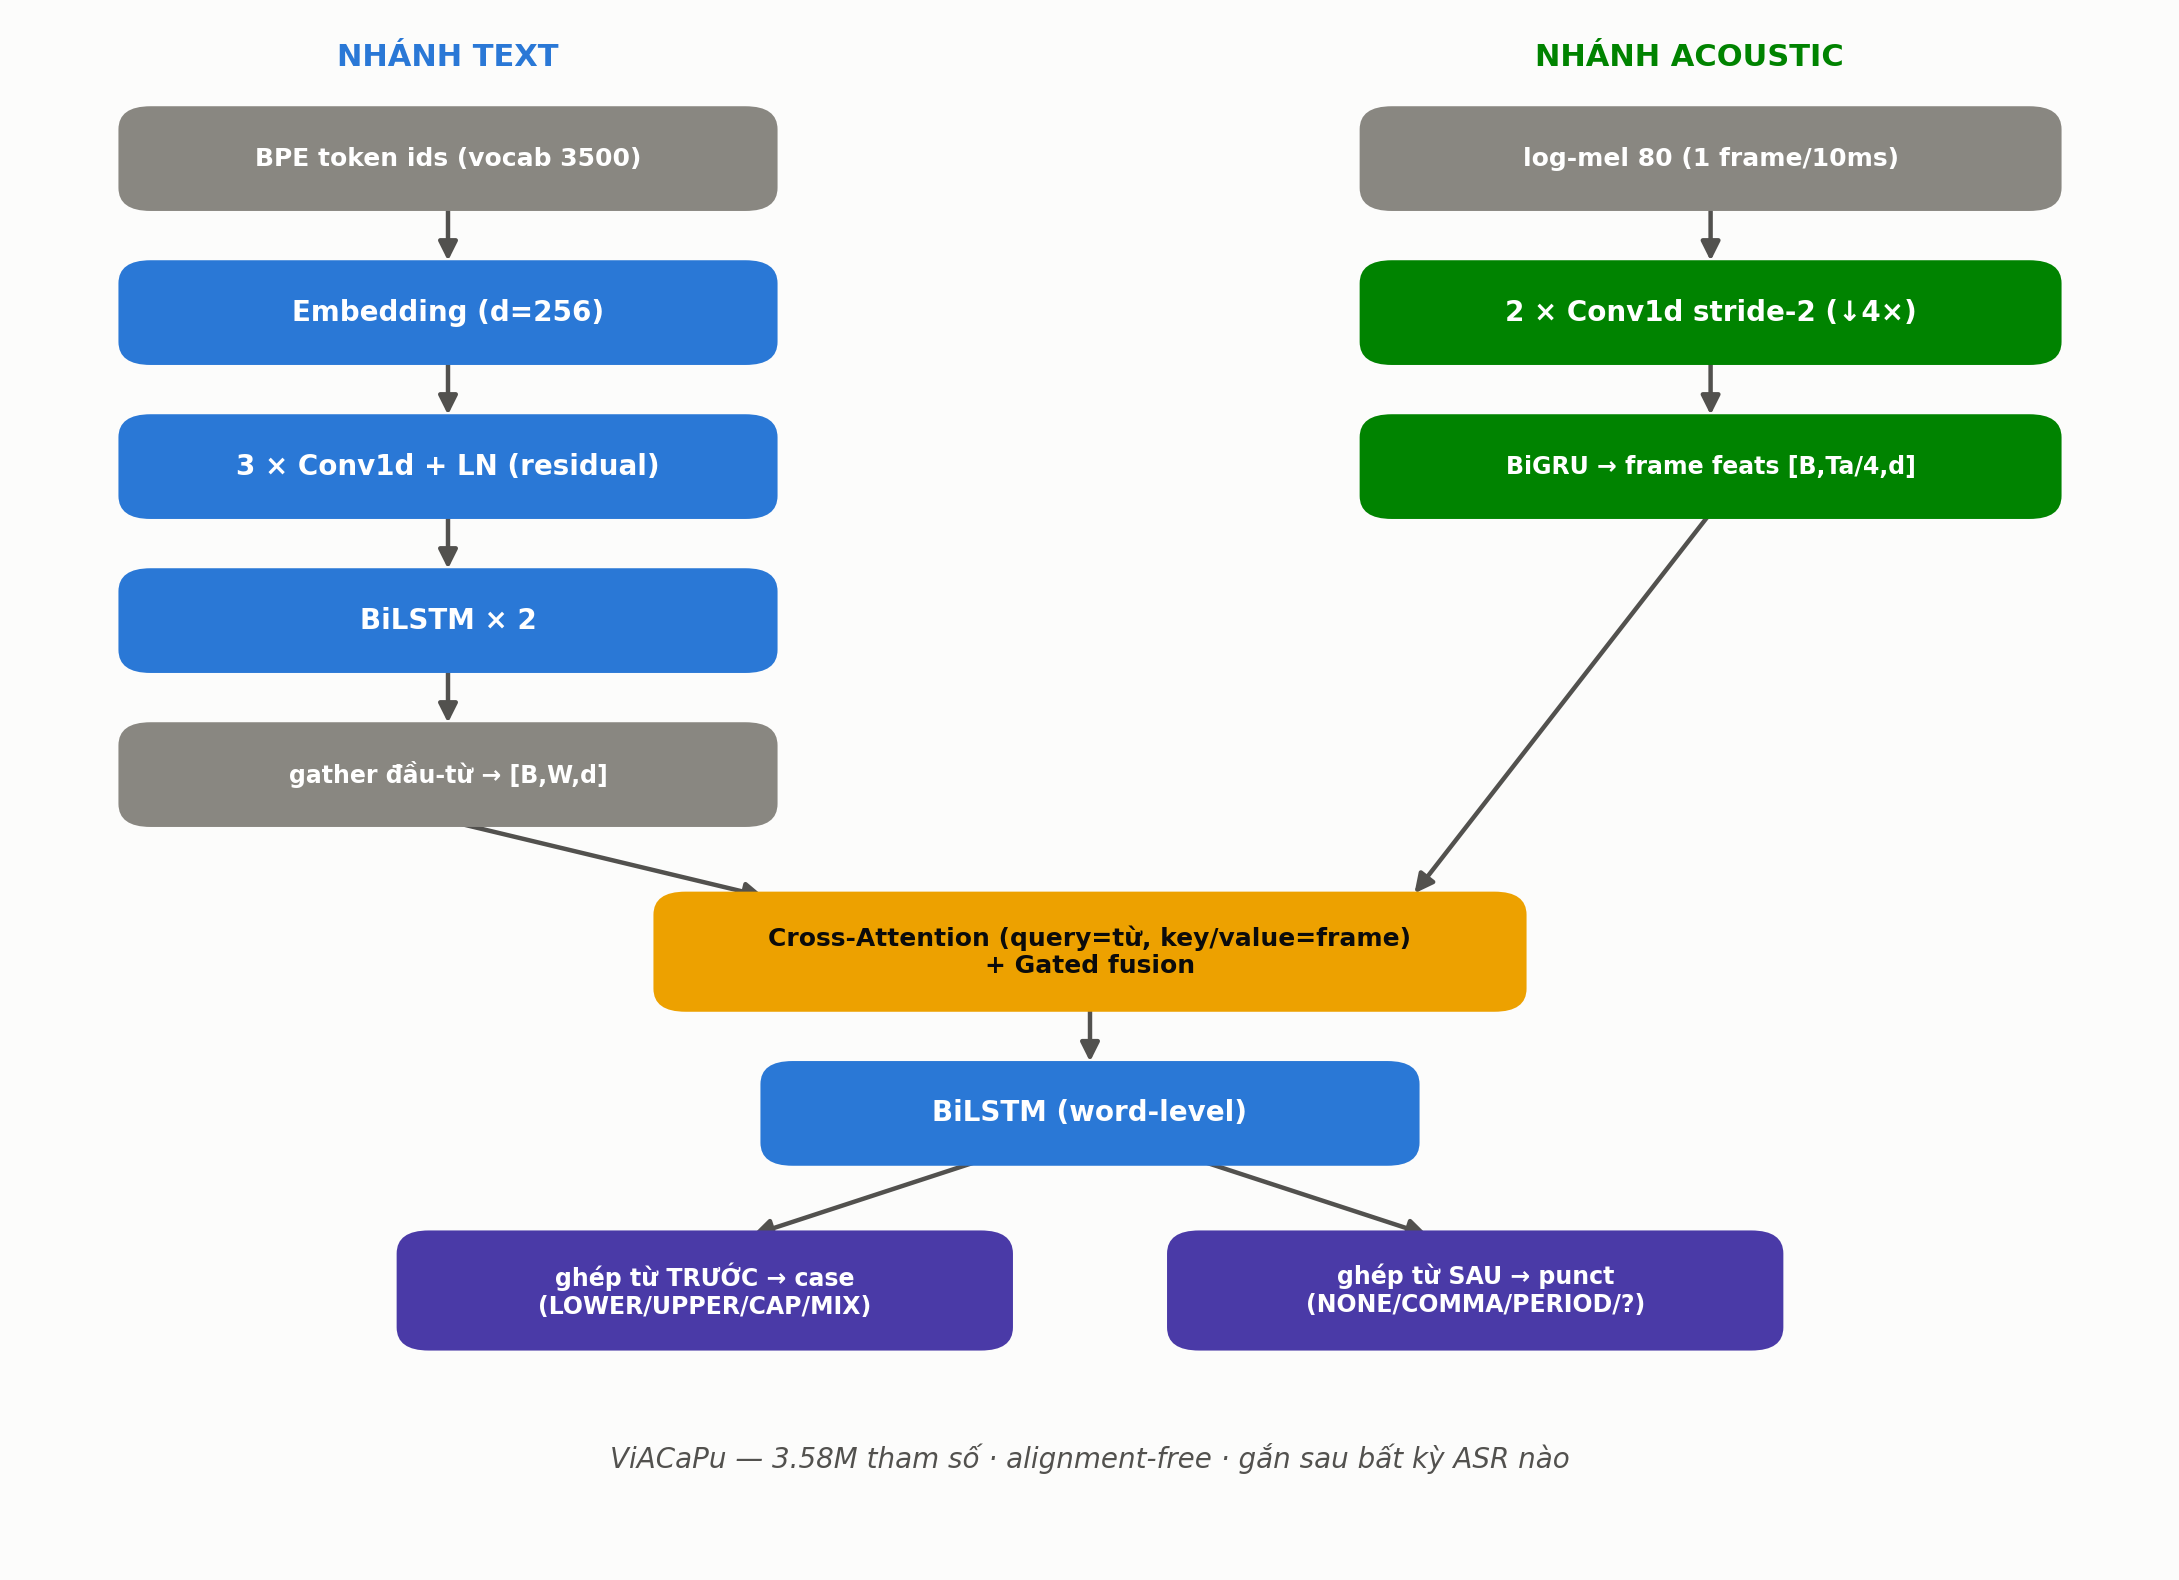
\includegraphics[width=\columnwidth]{figures/fig0_architecture.png}}
\caption{ViACaPu architecture. The text branch (left) and the acoustic branch
(right) are combined by gated cross-attention; the casing head observes the
preceding word state and the punctuation head the following one.}
\label{fig:arch}
\end{figure}

Fig.~\ref{fig:arch} depicts the model. We use $d=256$ throughout.

\subsection{Text branch}
BPE token identifiers (vocabulary 3500) are embedded and processed by three
residual \mbox{Conv1d} blocks ($k=3$, LayerNorm) followed by a two-layer BiLSTM.
Only the first sub-word of each word---marked by a validity mask---is retained,
yielding word-level states $\mathbf{H}^{t} \in \mathbb{R}^{B \times W \times d}$.

\subsection{Acoustic branch}
The 80-dimensional log-Mel spectrogram (10\,ms hop) is downsampled by two stride-2
convolutions ($4\times$ temporal reduction) and encoded by a BiGRU, producing frame
features $\mathbf{A} \in \mathbb{R}^{B \times T_a/4 \times d}$. An auxiliary head
predicts per-frame energy, encouraging the encoder to represent pauses and
dynamics. No alignment with the text is required.

\subsection{Gated cross-attention fusion}
Each word state queries the acoustic frames:
\begin{align}
\mathbf{C} &= \mathrm{CrossAttn}(\mathbf{Q}{=}\mathbf{H}^{t},\;
              \mathbf{K}{=}\mathbf{V}{=}\mathbf{A}), \\
\mathbf{Z} &= \sigma\!\left(\mathbf{W}\,[\mathbf{H}^{t};\mathbf{C}] + \mathbf{b}\right), \\
\mathbf{H}^{f} &= \mathbf{Z}\odot\mathbf{H}^{t} + (\mathbf{1}-\mathbf{Z})\odot\mathbf{C}.
\end{align}
Here $\mathbf{H}^{t}\!\in\!\mathbb{R}^{B\times W\times d}$ are the word-level
representations from the text branch (\S B), used as the \emph{query}, and
$\mathbf{A}\!\in\!\mathbb{R}^{B\times T_a/4\times d}$ are the frame features from
the acoustic branch (\S C), used as \emph{key} and \emph{value}.
$\mathrm{CrossAttn}$ is standard multi-head cross-attention, yielding a per-word
acoustic context $\mathbf{C}$. $[\,\cdot\,;\,\cdot\,]$ denotes feature-wise
concatenation; $\mathbf{W}\!\in\!\mathbb{R}^{d\times 2d}$ and
$\mathbf{b}\!\in\!\mathbb{R}^{d}$ are the gate weight and bias; $\sigma$ is the
element-wise sigmoid; $\odot$ is the Hadamard (element-wise) product. The learned
gate $\mathbf{Z}\!\in\![0,1]^{B\times W\times d}$ lets the model decide, per word
and per dimension, how much to trust acoustic evidence: when acoustics are
unreliable (noise, overlapping speech), $\mathbf{Z}\!\to\!1$ and the fused
representation $\mathbf{H}^{f}$ falls back to $\mathbf{H}^{t}$, keeping the model
robust. ($B$: batch size; $W$: number of words; $T_a$: number of acoustic frames;
$d$: hidden size.)

\subsection{Output heads and objective}
A word-level BiLSTM is followed by two linear heads. Following
\cite{you2024lightweight}, the casing head consumes $[\mathbf{h}_{i-1};\mathbf{h}_i]$
(left context determines capitalisation) and the punctuation head
$[\mathbf{h}_i;\mathbf{h}_{i+1}]$ (the next word signals a boundary). Both predict
four classes: casing $\in$ \{LOWER, UPPER, CAP, MIX\} and punctuation $\in$
\{NONE, COMMA, PERIOD, QUESTION\}, where ``!''$\rightarrow$PERIOD and
``;'',``:''$\rightarrow$COMMA. Here $\mathbf{h}_i$ is the word-level BiLSTM state
at word position $i$. The objective is
\begin{equation}
\mathcal{L} = \mathcal{L}_{\mathrm{CE}}^{\mathrm{case}}
            + 0.7\,\mathcal{L}_{\mathrm{CE}}^{\mathrm{punct}}(\mathbf{w}),
\end{equation}
where $\mathcal{L}_{\mathrm{CE}}^{\mathrm{case}}$ and
$\mathcal{L}_{\mathrm{CE}}^{\mathrm{punct}}$ are the cross-entropy losses of the
two tasks (computed only over real word positions, excluding padding);
$\mathbf{w}=[1.0,1.6,1.05,1.4]$ are the punctuation class weights for [NONE, COMMA,
PERIOD, QUES], counteracting the scarcity of COMMA and QUESTION; the coefficient
$0.7$ balances the two tasks (\S IV-E).

\subsection{Parameter budget}
Table~\ref{tab:params} reports the per-module distribution. The acoustic encoder and
the fusion block together account for only 0.91M parameters.

\begin{table}[t]
\caption{Parameter distribution of ViACaPu ($d=256$).}
\label{tab:params}
\centering
\begin{tabular}{lrr}
\toprule
Module & Parameters & Share \\
\midrule
Embedding ($3500\times256$)      & 896{,}000  & 25.0\,\% \\
Text BiLSTM (2 layers)           & 790{,}528  & 22.1\,\% \\
Text Conv $\times3$ + LayerNorm  & 592{,}128  & 16.5\,\% \\
Acoustic encoder                 & 512{,}897  & 14.3\,\% \\
Word-level BiLSTM                & 395{,}264  & 11.0\,\% \\
Fusion (cross-attention + gate)  & 394{,}496  & 11.0\,\% \\
Output heads                     & 2{,}056    & \phantom{0}0.1\,\% \\
\midrule
\textbf{Total}                   & \textbf{3{,}583{,}369} & 100\,\% \\
\bottomrule
\end{tabular}
\end{table}

\section{Experimental Setup}

\textbf{Data source.} We use the public Vietnamese speech corpus
\emph{Dolly-1000h}\footnote{\texttt{dolly-vn/dolly-audio-1000h-vietnamese} on
HuggingFace.}, consisting of (audio, punctuated transcript) pairs across many
domains. After filtering overly short/long clips, the dataset has
\textbf{658{,}128 clips} ($\approx$973 h of audio, 15.3M words), split 98/2 into
train/validation with seed 42 (Table~\ref{tab:data}).

\textbf{Label generation.} From each punctuated transcript we tokenise into words
and assign two labels per word. The casing label follows the word's surface form
(LOWER/UPPER/CAP/MIX); the punctuation label is the mark \emph{following} the word,
where ``!''$\rightarrow$PERIOD and ``;'',``:''$\rightarrow$COMMA to fold into four
classes. The (lowercased, de-punctuated) text is tokenised with SentencePiece BPE
(vocabulary 3500); only each word's first sub-word carries a label, the rest are
masked. The label distribution is strongly imbalanced (Table~\ref{tab:data}); in
particular QUESTION is only 0.23\,\%, motivating the class weighting in Eq.~(4).

\textbf{Acoustic features.} Audio is resampled to 16\,kHz and converted to
80-dimensional log-Mel spectrograms (25\,ms window, 10\,ms hop; \texttt{n\_fft}=400,
\texttt{hop}=160), then per-utterance mean--variance normalised. The frame sequence
is downsampled $4\times$ by the acoustic branch (Section~\ref{sec:method}).

\begin{table}[t]
\caption{Statistics of the Dolly-1000h corpus used in this work.}
\label{tab:data}
\centering
\small
\setlength{\tabcolsep}{4pt}
\begin{tabular}{lr}
\toprule
Attribute & Value \\
\midrule
Clips (train / val)         & 644{,}966 / 13{,}162 \\
Total audio duration        & $\approx$973 h \\
Clip length (mean / max)    & 5.3 / 16.0\,s \\
Total labelled words        & 15.3M \\
\midrule
PUNCT freq.\ (\%) & \\
\quad NONE / COMMA / PERIOD / QUES & 91.6 / 3.7 / 4.5 / 0.2 \\
CASE freq.\ (\%) & \\
\quad LOWER / UPPER / CAP / MIX    & 92.4 / 0.1 / 7.5 / 0.01 \\
\bottomrule
\end{tabular}
\end{table}

\textbf{Training.} Adam, learning rate $8\times10^{-4}$, weight decay
$5\times10^{-5}$, cosine annealing over 12 epochs, batch size 64. A single NVIDIA
RTX~3060 (12\,GB) trains ViACaPu in about 1.5 h.

\textbf{Metrics.} Word-level micro precision, recall and F1 per class; the overall
score aggregates the three non-NONE punctuation classes.

\textbf{Baselines.} (a)~The text-only model of~\cite{you2024lightweight} (7.26M
parameters), retrained on Dolly for a same-domain comparison; (b)~ViACaPu with the
acoustic branch disabled (2.68M), an ablation sharing the text branch and heads
exactly.

\textbf{Justification of hyper-parameters.} The main choices are grounded rather
than arbitrary. (i)~\emph{Loss weight $0.7$}: inherited from the base
model~\cite{you2024lightweight}, whose authors swept $(0.5, 2)$ and found $0.7$
optimal; casing is the easier task and thus warrants a smaller weight on
punctuation. (ii)~\emph{Width $d=256$}: an empirically validated sweet spot.
Increasing to $d=384$ \emph{degrades} quality (punctuation F1 $0.921 \rightarrow
0.821$): the wider text branch converges before cross-attention learns the soft
alignment, so the gate closes and the acoustic branch stops contributing (a ``gate
collapse''). Thus $d=256$ is simultaneously smaller, highest-scoring, and
edge-friendly. (iii)~\emph{Class weights $[1.0,1.6,1.05,1.4]$}: inversely
proportional to class frequency---rare COMMA and QUESTION receive higher weights.
(iv)~The remaining optimisation hyper-parameters follow standard settings and were
not separately tuned.

\section{Results}
\label{sec:results}

\subsection{Overall comparison}

\begin{table}[t]
\caption{Results on Dolly (Vietnamese). Each model is evaluated in the input format
it was designed for; the strictly controlled comparison (same subset, same format)
is between the two ViACaPu variants.}
\label{tab:main}
\centering
\small
\setlength{\tabcolsep}{4pt}
\begin{tabular}{lrccc}
\toprule
Model & Params & Case F1 & Punct F1 & COMMA \\
\midrule
Baseline~\cite{you2024lightweight}   & 7.26M & 0.856 & 0.703 & 0.577 \\
ViACaPu (text-only)                  & 2.68M & 0.938 & 0.822 & 0.661 \\
\textbf{ViACaPu (acoustic)}          & \textbf{3.58M} & \textbf{0.943} & \textbf{0.921} & \textbf{0.873} \\
\bottomrule
\end{tabular}
\end{table}

Table~\ref{tab:main} and Fig.~\ref{fig:compare} summarise the main result. The core
contribution is a CaPu model that is \emph{both lightweight and high-quality} for
the edge; the acoustic branch is one of the methods---alongside class weighting and
a compact architecture---used to reach that goal. The most tightly controlled
comparison is between the two ViACaPu variants (same text branch, same heads, same
audio validation split, differing only in whether the acoustic branch is enabled):
the acoustic branch raises punctuation F1 by \textbf{+0.099} and comma F1 by
\textbf{+0.212} for only 0.91M additional parameters. Relative to the text-only
baseline of~\cite{you2024lightweight} retrained on the same Dolly data, ViACaPu is
also \emph{smaller} (3.58M vs.\ 7.26M) while scoring markedly higher.

\begin{figure}[t]
\centerline{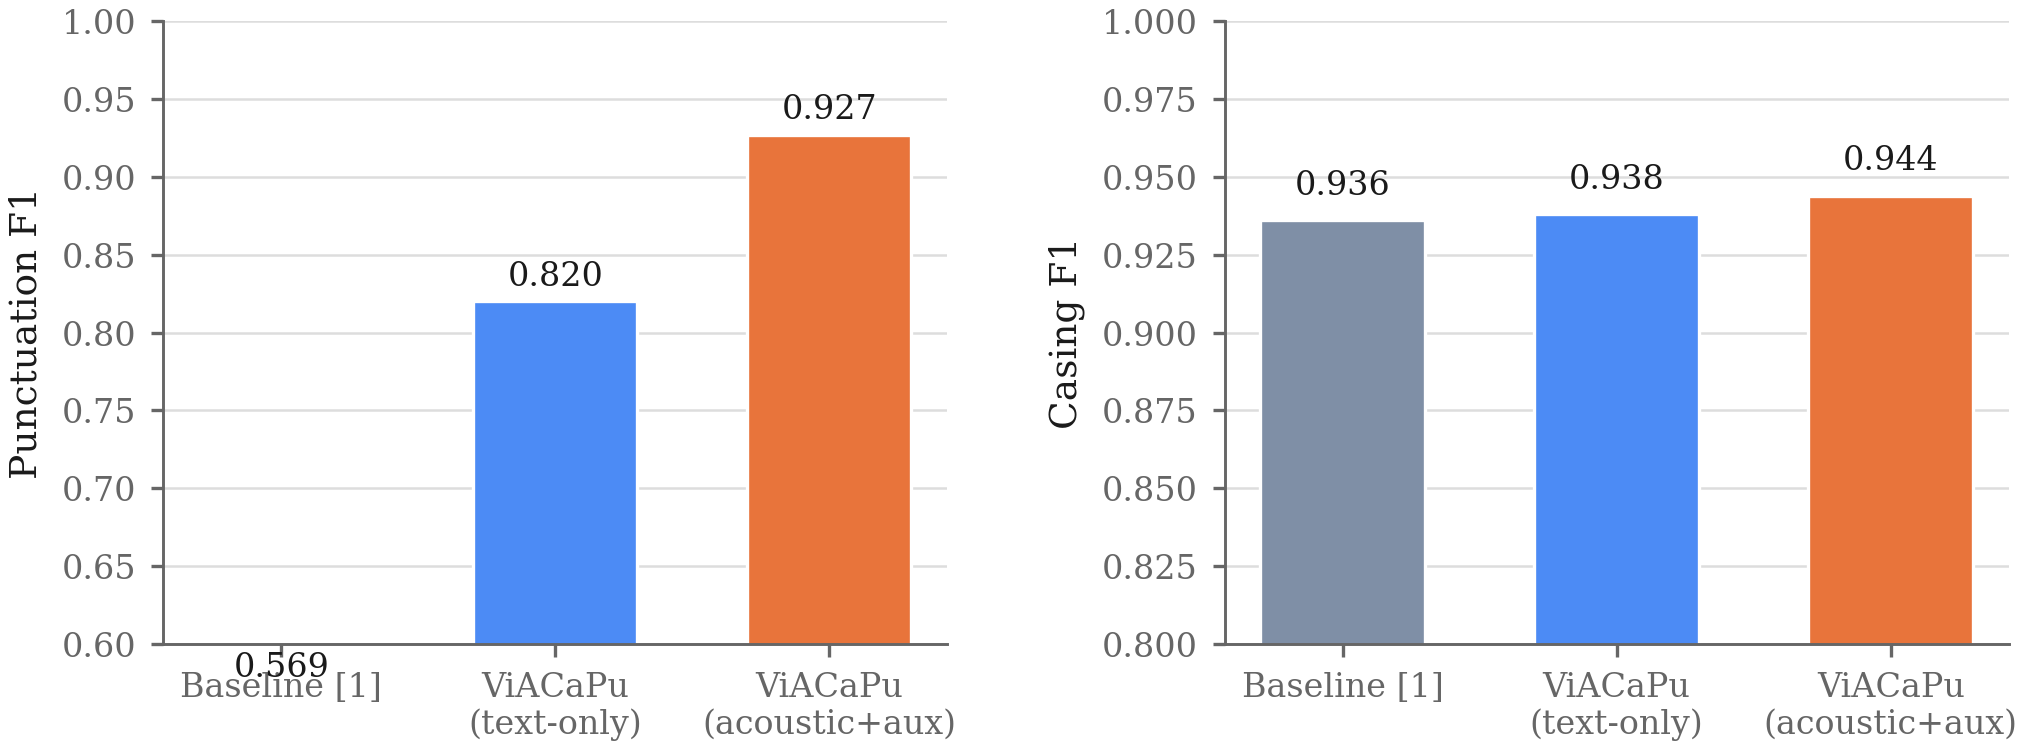
\includegraphics[width=\columnwidth]{figures/fig1_compare_all_models.png}}
\caption{Punctuation and casing F1 on Dolly. The baseline is evaluated on the text
test set and ViACaPu on the audio validation split; the strictly controlled
comparison is between the two ViACaPu variants.}
\label{fig:compare}
\end{figure}

\subsection{Per-class analysis}

\begin{table}[t]
\caption{Per-class punctuation results of ViACaPu (acoustic) on Dolly.}
\label{tab:perclass}
\centering
\begin{tabular}{lccc}
\toprule
Class & Precision & Recall & F1 \\
\midrule
COMMA        & 0.856 & 0.892 & 0.873 \\
PERIOD       & 0.982 & 0.956 & 0.969 \\
QUESTION     & 0.802 & 0.755 & 0.778 \\
\midrule
\textbf{Overall} & 0.920 & 0.923 & \textbf{0.921} \\
\bottomrule
\end{tabular}
\end{table}

Fig.~\ref{fig:perclass} and Table~\ref{tab:perclass} localise the improvement. The
confusion matrices in Fig.~\ref{fig:cmpunct} are more explicit: the text-only model
misses 33.5\,\% of all commas (predicting NONE), whereas the acoustic model misses
only 10.2\,\%---raising comma recall from 0.659 to 0.892. This is precisely the
behaviour the pause hypothesis predicts. Casing, in contrast, is essentially
unaffected (Fig.~\ref{fig:cmcase}), confirming that capitalisation is a
predominantly lexical phenomenon.

\begin{figure}[t]
\centerline{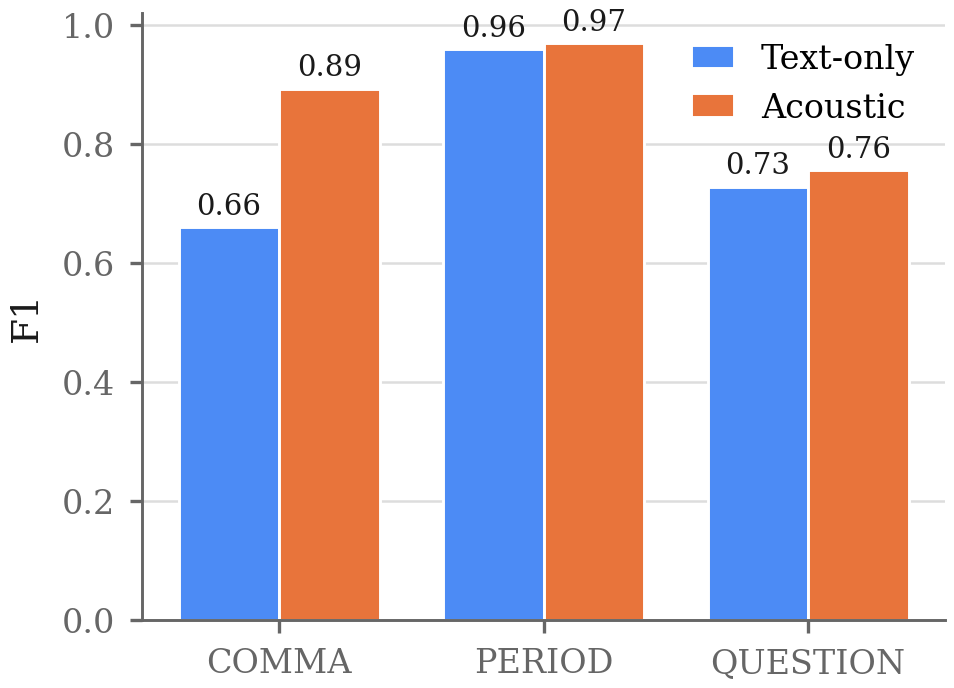
\includegraphics[width=\columnwidth]{figures/fig2_punct_f1_perclass.png}}
\caption{Per-class punctuation F1. The acoustic gain concentrates on COMMA.}
\label{fig:perclass}
\end{figure}

\begin{figure}[t]
\centerline{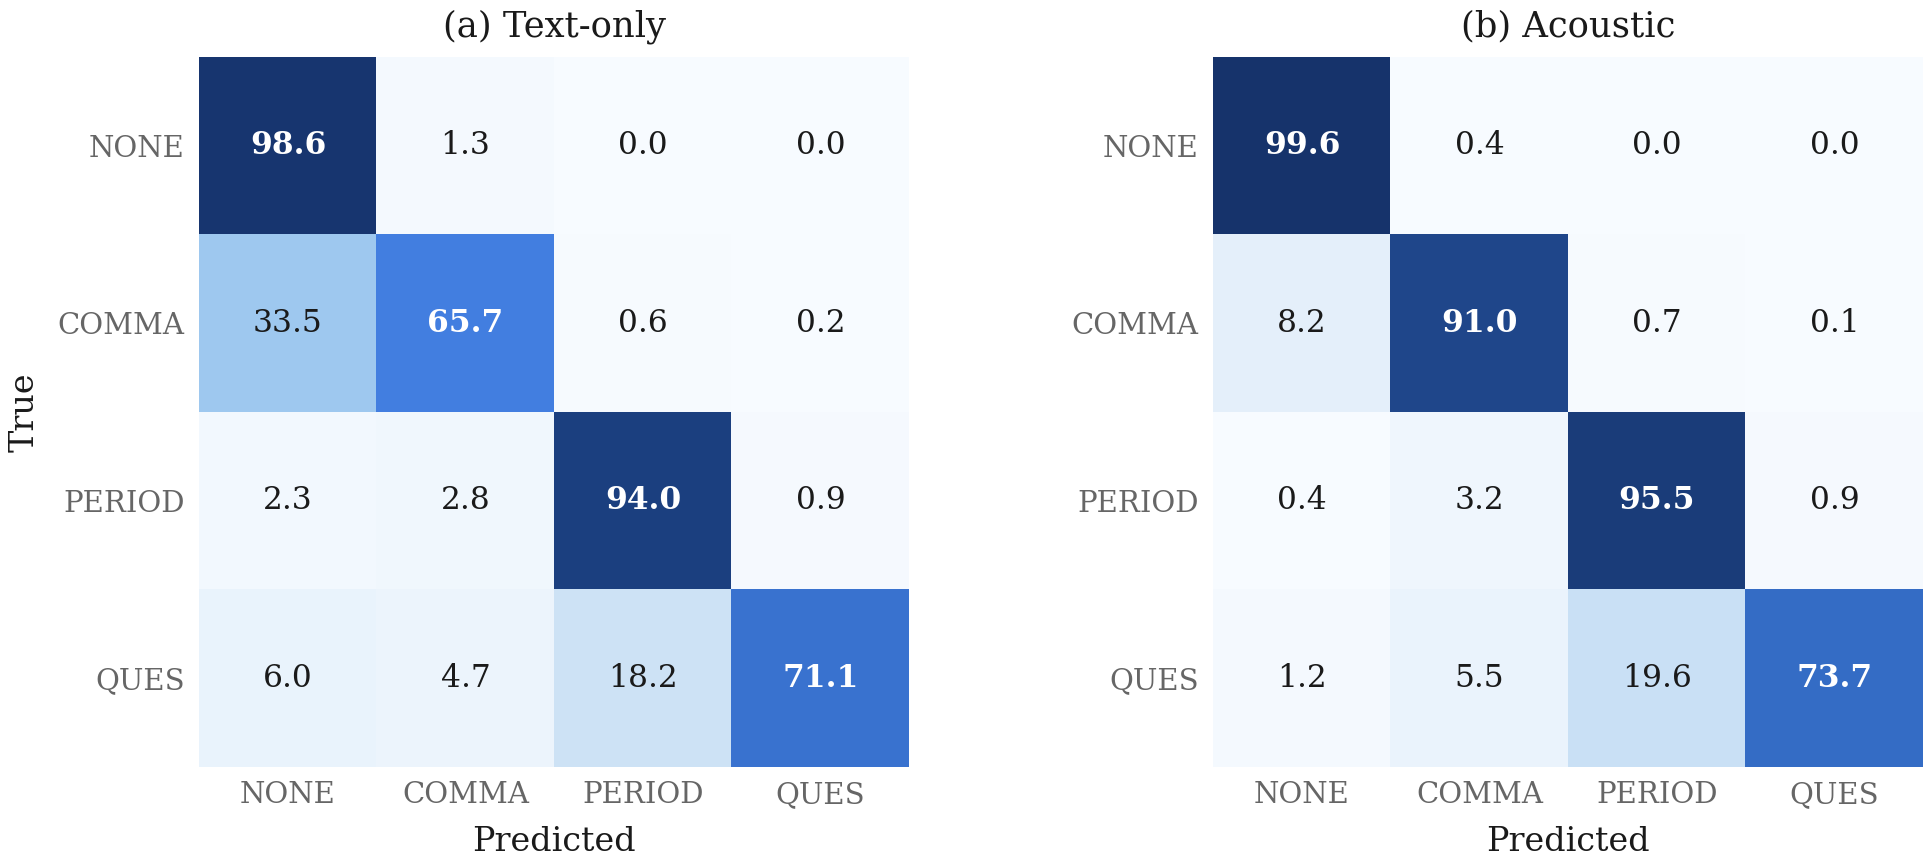
\includegraphics[width=\columnwidth]{figures/fig3_confusion_punct_acoustic.png}}
\caption{Punctuation confusion matrices (row-normalised). (a) Text-only vs.\
(b) acoustic; each cell reports the row percentage.}
\label{fig:cmpunct}
\end{figure}

\begin{figure}[t]
\centerline{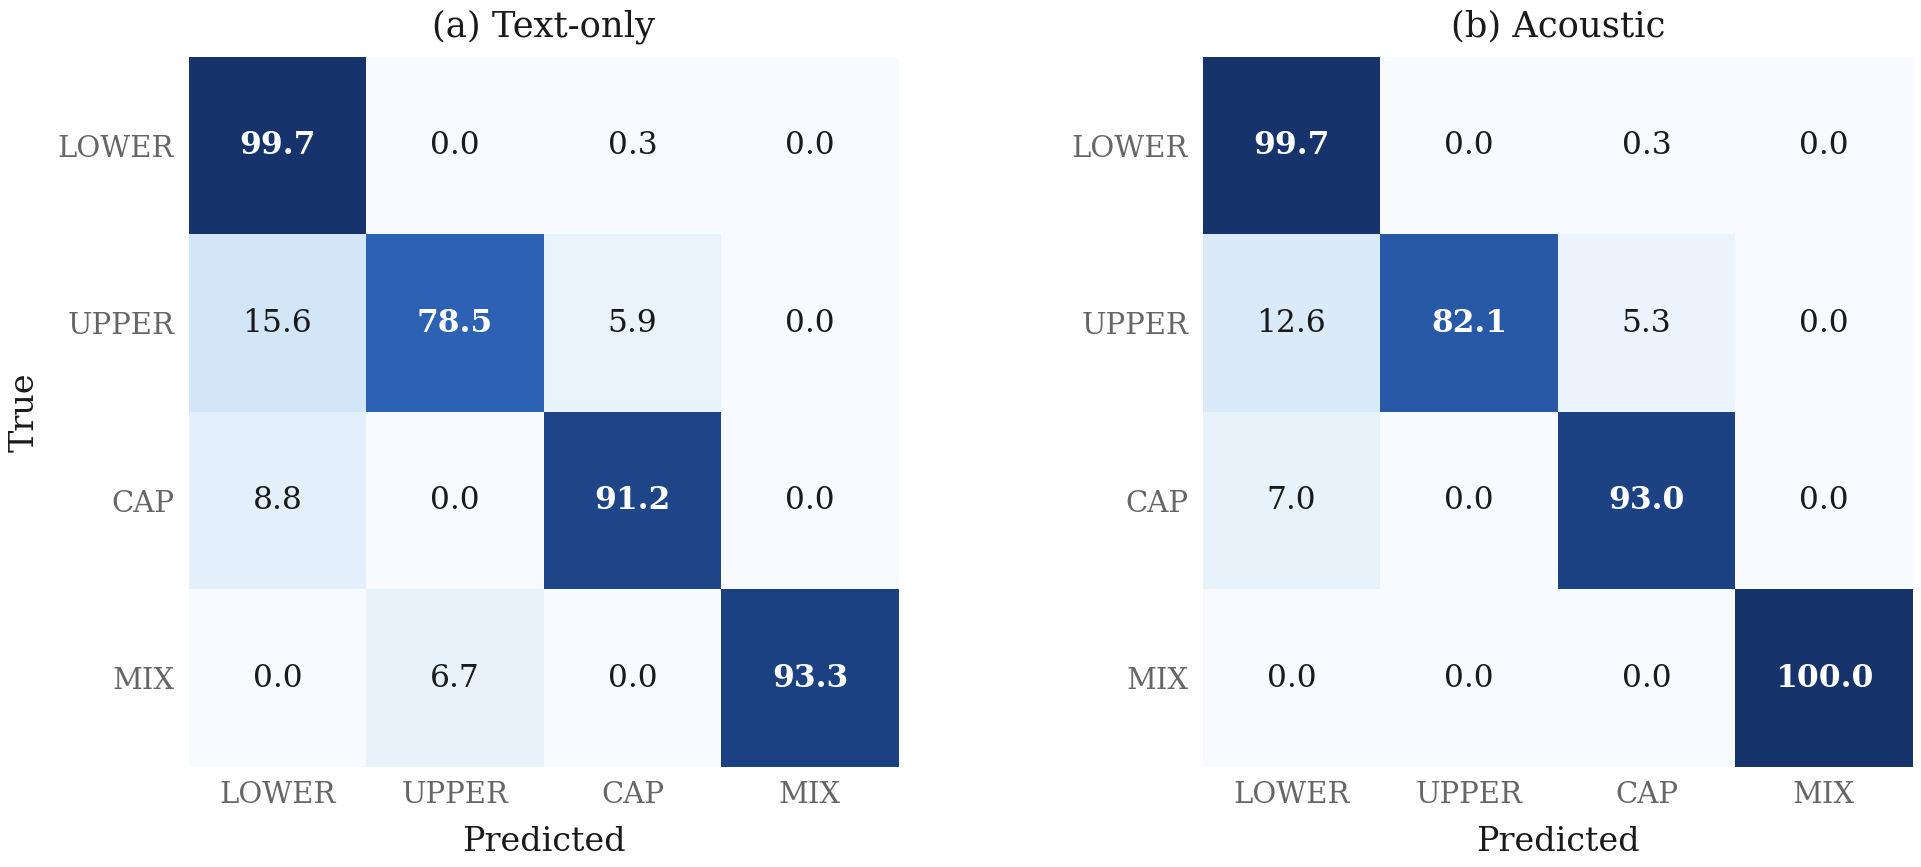
\includegraphics[width=\columnwidth]{figures/fig4_confusion_case_acoustic.png}}
\caption{Casing confusion matrices. The two variants are nearly identical.}
\label{fig:cmcase}
\end{figure}

\subsection{Effect of in-domain training}

\begin{figure}[t]
\centerline{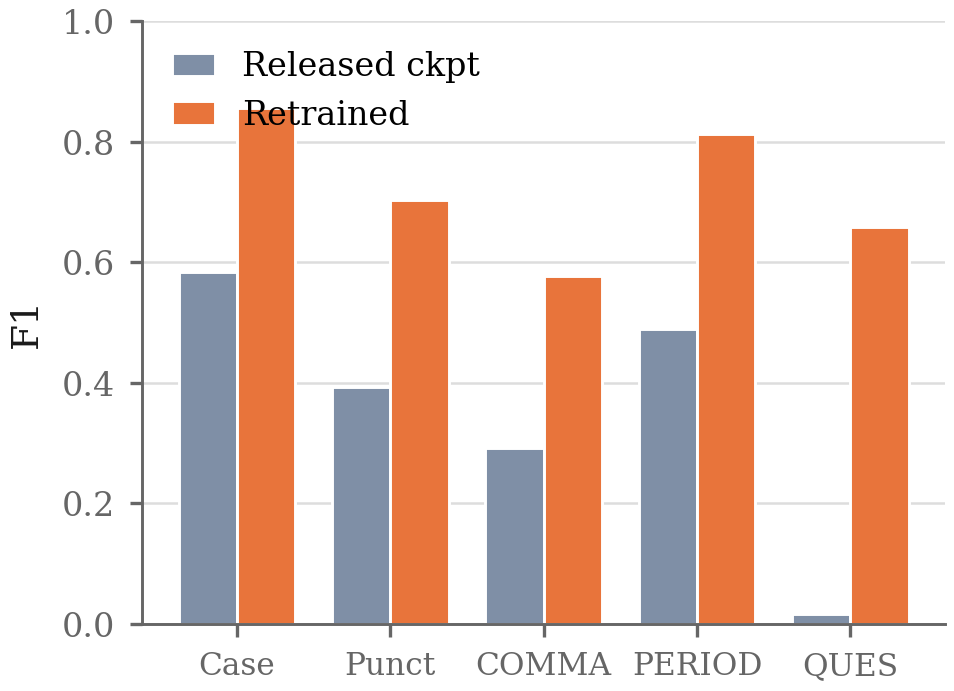
\includegraphics[width=\columnwidth]{figures/fig6_base_domain_shift.png}}
\caption{The released checkpoint of~\cite{you2024lightweight} vs.\ the same
architecture retrained on Dolly, both evaluated on the Dolly test set.}
\label{fig:domain}
\end{figure}

Fig.~\ref{fig:domain} quantifies domain shift: applied directly to Vietnamese, the
released baseline checkpoint attains only 0.393 punctuation F1 (QUESTION essentially
unrecognised); retraining the identical architecture on Dolly raises this to 0.703.
All comparisons in Table~\ref{tab:main} therefore use the retrained baseline.

\section{Discussion}

\textbf{Where prosody helps.} The improvement is not uniform across classes but
concentrates exactly where linguistic theory predicts. Commas, which co-occur with
pauses in spontaneous speech, gain $+0.212$ F1; questions, marked by a rising
terminal contour, gain $+0.037$; casing, determined by lexical and positional cues,
is unchanged. This correspondence between the observed gains and the prosodic nature
of each class supports the interpretation that the acoustic branch genuinely
exploits prosody rather than merely adding capacity.

\textbf{Cost--benefit for the edge.} The acoustic branch and fusion block together
add 0.91M parameters ($+34\,\%$ relative), buying $+0.099$ absolute punctuation F1.
The full model remains at 3.58M parameters---half the text-only baseline---and
converges in about 1.5 h on a single consumer GPU, so both memory and training
budget stay within edge reach.

\textbf{Design implications.} Two properties matter for practical integration.
First, the fusion is alignment-free, needing no word-level timestamps, so the module
attaches to a deployed recogniser unchanged. Second, the per-word gate lets the
model fall back on lexical evidence when the acoustic signal is unreliable (noise,
overlapping speech).

\textbf{Limitations.} Our evaluation covers a single language and speech domain; how
far the gains transfer depends on how faithfully a corpus punctuation convention
reflects the speaker's phrasing rather than editorial style. The QUESTION class
remains the weakest (F1 0.778), reflecting its scarcity (0.23\,\% of tokens).

\section{Conclusion}

We presented ViACaPu, a 3.58M-parameter acoustic-aware model for punctuation and
casing restoration that fuses text and log-Mel evidence through alignment-free gated
cross-attention and can be attached to any deployed ASR system. On Vietnamese
Dolly-1000h it improves punctuation F1 from 0.822 to 0.921 and comma F1 from 0.661
to 0.873 relative to an identically-configured text-only ablation, using only 0.91M
additional parameters while remaining smaller than the text-only baseline
of~\cite{you2024lightweight}. Error analysis confirms the gain is concentrated on
prosodically marked classes. Future work includes evaluation on further languages
and domains, joint multilingual training, and quantised on-device deployment.

\begin{thebibliography}{00}

\bibitem{you2024lightweight}
J.~You and X.~Li, ``A light-weight and efficient punctuation and word casing
prediction model for on-device streaming ASR,'' Cisco Systems, \emph{arXiv
preprint arXiv:2407.13142}, 2024.

\bibitem{unipunc}
Y.~Zhu, L.~Wu, S.~Cheng, and M.~Wang, ``Unified multimodal punctuation restoration
framework for mixed-modality corpus,'' in \emph{Proc. IEEE ICASSP}, 2022.

\bibitem{stpt}
A.~Jakubiak \emph{et al.}, ``Adapting ASR models for speech-to-punctuated-text
recognition with utterance gluing,'' Samsung R\&D Institute Poland, in
\emph{Proc. ICNLSP}, 2025.

\bibitem{jointcappunc}
H.~T.~T. Uyen, N.~A. Tu, and T.~D. Huy, ``Vietnamese capitalization and punctuation
recovery models,'' in \emph{Proc. INTERSPEECH}, 2022.

\bibitem{cho2022}
J.~Y. Cho, S.~Ng, T.~Tran, and M.~Ostendorf, ``Leveraging prosody for punctuation
prediction of spontaneous speech,'' in \emph{Proc. INTERSPEECH}, 2022.

\bibitem{tran2020}
X.~Che \emph{et al.}, ``Multimodal semi-supervised learning framework for
punctuation prediction in conversational speech,'' \emph{arXiv preprint
arXiv:2008.00702}, 2020.

\bibitem{bertpunct}
A.~Nagy, B.~Bial, and J.~\'Acs, ``Automatic punctuation restoration with BERT
models,'' \emph{arXiv preprint arXiv:2101.07343}, 2021.

\bibitem{survey}
V.~P\u{a}i\c{s} and D.~Tufi\c{s}, ``Capitalization and punctuation restoration:
a survey,'' \emph{Artificial Intelligence Review}, 2022.

\bibitem{polacek2023}
M.~Pol\'a\v{c}ek \emph{et al.}, ``Online punctuation restoration using ELECTRA
model for streaming ASR systems,'' in \emph{Proc. INTERSPEECH}, 2023.

\bibitem{lightweight2025}
``Lightweight online punctuation and capitalization restoration for streaming ASR
systems,'' \emph{Speech Communication}, 2025.

\bibitem{kim2023}
J.~Kim \emph{et al.}, ``Improved training for end-to-end streaming automatic
speech recognition model with punctuation,'' in \emph{Proc. INTERSPEECH}, 2023.

\bibitem{librispeechpc}
A.~Meister \emph{et al.}, ``LibriSpeech-PC: Benchmark for evaluation of
punctuation and capitalization capabilities of end-to-end ASR models,'' in
\emph{Proc. IEEE ASRU}, 2023.

\bibitem{nguyen2019}
B.~Nguyen \emph{et al.}, ``Fast and accurate capitalization and punctuation for
automatic speech recognition using transformer and chunk merging,'' in
\emph{Proc. O-COCOSDA}, 2019.

\bibitem{sunkara2020}
M.~Sunkara \emph{et al.}, ``Robust prediction of punctuation and truecasing for
medical ASR,'' in \emph{Proc. ACL Workshop on NLP for Medical Conversations},
2020.

\end{thebibliography}

\end{document}
